% Ring sampling window around a building footprint, with the property parcel
% P(b) and the street parcel S(b) the layered FIS also evaluates.
%
% Goes in the bottom-right cell of study_area_context.pdf, which
% paper_study_area_figure.py leaves empty for it (run that script and it prints
% the reserved cell's size in inches).
%
% Standalone so it can be compiled on its own:
%     pdflatex sampling_window_diagram.tex
% To use it inside the paper instead, \input only the tikzpicture below and
% keep \usetikzlibrary{calc} in the paper's preamble.
\documentclass[tikz,border=2pt]{standalone}
\usepackage{tikz}
\usetikzlibrary{calc}
\begin{document}
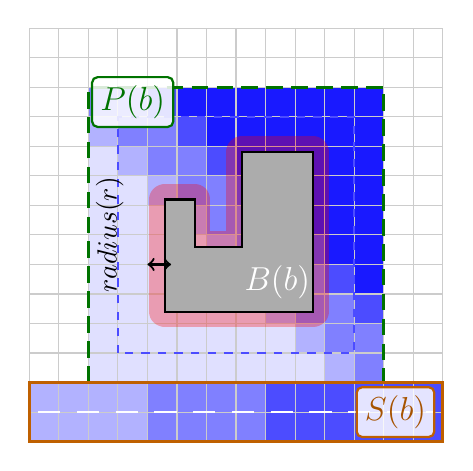
\begin{tikzpicture}[scale=0.75]

%--------------------------------------------------
% Raster grid
%--------------------------------------------------
\draw[step=0.5cm, gray!50] (0,0) grid (7,7);

%--------------------------------------------------
% Sampled raster cells inside sampling window, shaded by flood depth
%--------------------------------------------------
\fill[blue!12] (1.5,1.5) rectangle ++(0.5,0.5);
\fill[blue!12] (1.5,2.0) rectangle ++(0.5,0.5);
\fill[blue!12] (1.5,2.5) rectangle ++(0.5,0.5);
\fill[blue!12] (1.5,3.0) rectangle ++(0.5,0.5);
\fill[blue!12] (1.5,3.5) rectangle ++(0.5,0.5);
\fill[blue!12] (1.5,4.0) rectangle ++(0.5,0.5);
\fill[blue!30] (1.5,4.5) rectangle ++(0.5,0.5);
\fill[blue!50] (1.5,5.0) rectangle ++(0.5,0.5);
\fill[blue!12] (2.0,1.5) rectangle ++(0.5,0.5);
\fill[blue!12] (2.0,2.0) rectangle ++(0.5,0.5);
\fill[blue!12] (2.0,2.5) rectangle ++(0.5,0.5);
\fill[blue!12] (2.0,3.0) rectangle ++(0.5,0.5);
\fill[blue!12] (2.0,3.5) rectangle ++(0.5,0.5);
\fill[blue!30] (2.0,4.0) rectangle ++(0.5,0.5);
\fill[blue!50] (2.0,4.5) rectangle ++(0.5,0.5);
\fill[blue!50] (2.0,5.0) rectangle ++(0.5,0.5);
\fill[blue!12] (2.5,1.5) rectangle ++(0.5,0.5);
\fill[blue!12] (2.5,2.0) rectangle ++(0.5,0.5);
\fill[blue!12] (2.5,2.5) rectangle ++(0.5,0.5);
\fill[blue!12] (2.5,3.0) rectangle ++(0.5,0.5);
\fill[blue!30] (2.5,3.5) rectangle ++(0.5,0.5);
\fill[blue!50] (2.5,4.0) rectangle ++(0.5,0.5);
\fill[blue!50] (2.5,4.5) rectangle ++(0.5,0.5);
\fill[blue!70] (2.5,5.0) rectangle ++(0.5,0.5);
\fill[blue!12] (3.0,1.5) rectangle ++(0.5,0.5);
\fill[blue!12] (3.0,2.0) rectangle ++(0.5,0.5);
\fill[blue!12] (3.0,2.5) rectangle ++(0.5,0.5);
\fill[blue!30] (3.0,3.0) rectangle ++(0.5,0.5);
\fill[blue!50] (3.0,3.5) rectangle ++(0.5,0.5);
\fill[blue!50] (3.0,4.0) rectangle ++(0.5,0.5);
\fill[blue!70] (3.0,4.5) rectangle ++(0.5,0.5);
\fill[blue!90] (3.0,5.0) rectangle ++(0.5,0.5);
\fill[blue!12] (3.5,1.5) rectangle ++(0.5,0.5);
\fill[blue!12] (3.5,2.0) rectangle ++(0.5,0.5);
\fill[blue!30] (3.5,2.5) rectangle ++(0.5,0.5);
\fill[blue!50] (3.5,3.0) rectangle ++(0.5,0.5);
\fill[blue!50] (3.5,3.5) rectangle ++(0.5,0.5);
\fill[blue!70] (3.5,4.0) rectangle ++(0.5,0.5);
\fill[blue!90] (3.5,4.5) rectangle ++(0.5,0.5);
\fill[blue!90] (3.5,5.0) rectangle ++(0.5,0.5);
\fill[blue!12] (4.0,1.5) rectangle ++(0.5,0.5);
\fill[blue!30] (4.0,2.0) rectangle ++(0.5,0.5);
\fill[blue!50] (4.0,2.5) rectangle ++(0.5,0.5);
\fill[blue!50] (4.0,3.0) rectangle ++(0.5,0.5);
\fill[blue!70] (4.0,3.5) rectangle ++(0.5,0.5);
\fill[blue!90] (4.0,4.0) rectangle ++(0.5,0.5);
\fill[blue!90] (4.0,4.5) rectangle ++(0.5,0.5);
\fill[blue!90] (4.0,5.0) rectangle ++(0.5,0.5);
\fill[blue!30] (4.5,1.5) rectangle ++(0.5,0.5);
\fill[blue!50] (4.5,2.0) rectangle ++(0.5,0.5);
\fill[blue!50] (4.5,2.5) rectangle ++(0.5,0.5);
\fill[blue!70] (4.5,3.0) rectangle ++(0.5,0.5);
\fill[blue!90] (4.5,3.5) rectangle ++(0.5,0.5);
\fill[blue!90] (4.5,4.0) rectangle ++(0.5,0.5);
\fill[blue!90] (4.5,4.5) rectangle ++(0.5,0.5);
\fill[blue!90] (4.5,5.0) rectangle ++(0.5,0.5);
\fill[blue!50] (5.0,1.5) rectangle ++(0.5,0.5);
\fill[blue!50] (5.0,2.0) rectangle ++(0.5,0.5);
\fill[blue!70] (5.0,2.5) rectangle ++(0.5,0.5);
\fill[blue!90] (5.0,3.0) rectangle ++(0.5,0.5);
\fill[blue!90] (5.0,3.5) rectangle ++(0.5,0.5);
\fill[blue!90] (5.0,4.0) rectangle ++(0.5,0.5);
\fill[blue!90] (5.0,4.5) rectangle ++(0.5,0.5);
\fill[blue!90] (5.0,5.0) rectangle ++(0.5,0.5);

%--------------------------------------------------
% Depth shade as a function of position, matching the gradient above
% (the shade of every cell above is a function of x+y alone)
%--------------------------------------------------
\def\depthlevel#1#2{%
    \pgfmathtruncatemacro{\lvl}{%
        (#1+#2) < 6.0 ? 12 : ((#1+#2) < 6.5 ? 30 : ((#1+#2) < 7.5 ? 50 : ((#1+#2) < 8.0 ? 70 : 90)))%
    }%
}

%--------------------------------------------------
% Cells of the property parcel lying outside the building sampling window
%--------------------------------------------------
\foreach \x in {1.0,1.5,...,5.5}{
    \foreach \y in {1.0,1.5,...,5.5}{
        \pgfmathtruncatemacro{\outsidewindow}{%
            (\x < 1.4 || \x > 5.1 || \y < 1.4 || \y > 5.1) ? 1 : 0%
        }
        \ifnum\outsidewindow=1
            \depthlevel{\x}{\y}
            \fill[blue!\lvl] (\x,\y) rectangle ++(0.5,0.5);
        \fi
    }
}

%--------------------------------------------------
% Cells of the street corridor. The road corridor sits lower than the
% surrounding land and ponds accordingly, so it carries its own depth
% gradient rather than the diagonal one used across the parcel.
%--------------------------------------------------
\foreach \x in {0,0.5,...,6.5}{
    \foreach \y in {0,0.5}{
        \pgfmathtruncatemacro{\slvl}{ \x < 2.0 ? 30 : (\x < 4.0 ? 50 : 70) }
        \fill[blue!\slvl] (\x,\y) rectangle ++(0.5,0.5);
    }
}

% Restore the cell boundaries over the shaded areas
\draw[step=0.5cm, gray!40] (0,0) grid (7,7);

%--------------------------------------------------
% Sampling window
%--------------------------------------------------
\draw[blue!70,dashed,thick] (1.5,1.5) rectangle (5.5,5.5);

%--------------------------------------------------
% Remove sampled cells inside building footprint
%--------------------------------------------------
\fill[white] (2.3,2.2) -- (4.8,2.2) -- (4.8,4.9) -- (3.6,4.9) -- (3.6,3.3) -- (2.8,3.3) -- (2.8,4.1) -- (2.3,4.1) -- cycle;

%--------------------------------------------------
% Building footprint
%--------------------------------------------------
\def\building{
    (2.3,2.2) --
    (4.8,2.2) --
    (4.8,4.9) --
    (3.6,4.9) --
    (3.6,3.3) --
    (2.8,3.3) --
    (2.8,4.1) --
    (2.3,4.1) -- cycle
}

% Buffer width = 2r
\draw[
    red!,
    opacity=0.3,
    line width=4mm,   % adjust to your desired radius
    line join=round,
    line cap=round
] \building;

% Remove the inside of the buffer
\fill[white] \building;



% Draw the building
\fill[gray!65] \building;
\draw[black,thick] \building;

% Radius r
\draw[<->,thick]
    (2.4,3.0) -- ++(-4mm,0);
\node[font=\normalsize, rotate=90] at (1.36,3.5){$radius(r)$};

%--------------------------------------------------
% Property parcel P(b)
%--------------------------------------------------
\draw[green!45!black, very thick, dash pattern=on 6pt off 3pt]
    (1,1) rectangle (6,6);

%--------------------------------------------------
% Street (road parcel) S(b)
%--------------------------------------------------
\draw[orange!75!black, very thick] (0,0) rectangle (7,1);
\draw[white, thick, dash pattern=on 8pt off 6pt] (0.15,0.5) -- (6.85,0.5);

%--------------------------------------------------
% Labels
%--------------------------------------------------
\node[white, font=\large\bfseries] at (4.2,2.7) {$B(b)$};

\node[green!45!black, font=\large\bfseries, fill=white, fill opacity=0.85,
      text opacity=1, draw=green!45!black, thick, rounded corners=2pt,
      inner sep=3pt] at (1.75,5.75) {$P(b)$};

\node[orange!65!black, font=\large\bfseries, fill=white, fill opacity=0.85,
      text opacity=1, draw=orange!75!black, thick, rounded corners=2pt,
      inner sep=3pt] at (6.2,0.5) {$S(b)$};

\end{tikzpicture}
\end{document}
